% ICML 2027 Two-Column Double-Blind Submission Draft
% Swap preamble to `\usepackage{icml2027}` once the official ICML 2027 style kit opens on Jan 8, 2027.
\documentclass[10pt,twocolumn]{article}
\usepackage[letterpaper,top=0.85in,bottom=0.85in,left=0.68in,right=0.68in,columnsep=0.25in]{geometry}
\usepackage[T1]{fontenc}
\usepackage{times}
\usepackage{natbib}
\setcitestyle{authoryear,round,citesep={;},aysep={,},yysep={;}}
\usepackage{fancyhdr}
\pagestyle{fancy}
\fancyhf{}
\lhead{\small\itshape Double-Blind Submission Draft (ICML 2027 Two-Column Format)}
\cfoot{\thepage}
\usepackage{amsmath,amssymb,amsthm,mathtools}
\usepackage{booktabs}
\usepackage{graphicx}
\usepackage{microtype}
\usepackage{xcolor}
\usepackage{enumitem}
\usepackage{url}
\usepackage[hidelinks]{hyperref}

\newtheorem{theorem}{Theorem}
\newtheorem{proposition}{Proposition}
\newtheorem{remark}{Remark}

\setlist[itemize]{leftmargin=1.4em,itemsep=2pt,topsep=3pt}
\newcommand{\KL}{D_{\mathrm{KL}}}

\title{\Large\bfseries Margin-Gated Probabilistic Surrogate Gradients for Overcomplete Sparse Autoencoders}
\author{Anonymous Authors \\ \textit{Paper under double-blind review}}
\date{}
\begin{document}
\maketitle
\begin{abstract}
Sparse Autoencoders (SAEs) trained with hard TopK or BatchTopK activations rely on straight-through estimators (STE) that assign identically zero gradient to inactive dictionary atoms, driving severe dead-latent collapse at high expansion factors (up to 78.6\% dead atoms at $4\times$ and 75.5\% at $8\times$ overcompleteness). Drawing on calibrated marginal subset routing from probabilistic Mixture-of-Experts, we first prove formally why naive full-backward probabilistic replacement (ProbBatchTopK v1) degrades reconstruction fidelity: multiplying active top-$k$ gradients by sigmoid derivatives distorts feature magnitudes. We introduce \textbf{MarginProb-BatchTopK}, which preserves exact identity STE gradients on the active top-$k$ set while routing scale-invariant calibrated marginal inclusion probabilities $p_{ij} = \sigma((z_{ij} - \tau)/(\tau_{\mathrm{rel}}\,\mathrm{std}(z)))$ exclusively to near-margin inactive latents. Across 9 $L_0$-matched SAE architectures at $4\times$ ($d_{\mathrm{sae}}=8{,}192$) and $8\times$ ($d_{\mathrm{sae}}=16{,}384$) overcompleteness on Qwen3-1.7B L13 and SmolLM2-1.7B L12 (205,883 leak-free paper-disjoint tokens, $k \in \{16,32,64\}$, 3 seeds), active-set gating completely eliminates v1's FVU penalty ($\Delta\mathrm{FVU} = -0.01569$, paired $t$-test $p=1.95e-09$). Against pure-MSE BatchTopK-STE, MarginProb-BatchTopK simultaneously lowers FVU (-0.00470, $p=4.10e-03$) and slashes dead latents by -19.90 pp ($p=7.69e-09$) with zero auxiliary loss. Splicing trained $k=32$ SAEs back into the live transformers confirms causal fidelity: MarginProb-BatchTopK recovers 98.82\% CE loss on SmolLM2-1.7B (KL $=0.2561$; MarginProb+AuxK 98.85\% / KL $=0.2552$, \#1 of all 9 methods) and 97.96\% on Qwen3-1.7B (eliminating ungated v1's drop to 97.20\%). At $8\times$ width ($d_{\mathrm{sae}}=16{,}384$), pure-MSE MarginProb ties the best FVU (0.2764) while cutting dead latents from 75.5\% (BatchTopK-STE) and 60.4\% (BatchTopK+AuxK) down to 54.9\%.
\end{abstract}


\section{Introduction}
Sparse Autoencoders (SAEs) decompose polysemantic transformer residual streams into sparse, interpretable features \citep{bricken2023monosemanticity,cunningham2024sae}. Modern architectures replace $L_1$-penalized ReLU SAEs with hard sparsity operators---TopK \citep{gao2024scaling}, BatchTopK \citep{bussmann2024batchtopk}, and JumpReLU \citep{rajamanoharan2024jumprelu}---to eliminate $L_1$ shrinkage bias. However, hard TopK/BatchTopK relies on straight-through estimators (STE; \citealt{bengio2013ste}) that route identically zero gradient to every unselected feature, driving severe dead-latent collapse at overcomplete widths and complicating cross-seed stability \citep{paulo2025sae}.

Drawing on calibrated marginal subset routing from probabilistic Mixture-of-Experts \citep{probmoe2026}, we diagnose why naive full-backward probabilistic replacement degrades reconstruction FVU and propose \textbf{MarginProb-BatchTopK}, which partitions the backward pass strictly on the active mask $M$. We evaluate 9 $L_0$-matched SAE architectures at $4\times$ ($d_{\mathrm{sae}}=8{,}192$) and $8\times$ ($d_{\mathrm{sae}}=16{,}384$) overcompleteness across two distinct 1.7B LLM families using held-out FVU, dead-latent rate, \textbf{live transformer causal splice CE Loss Recovered \& Logit KL}, downstream 8-class probe recovery, and capacity-controlled Top-512 Hungarian cross-seed matching.

\section{Diagnosis and MarginProb-BatchTopK Formulation}
Let $x \in \mathbb{R}^d$, pre-activation $z = (x - b_{\mathrm{dec}})W_{\mathrm{enc}} + b_{\mathrm{enc}} \in \mathbb{R}^M$, and hard BatchTopK mask $M \in \{0,1\}^{B\times M}$ selecting the $B\cdot k$ largest positive entries across a batch. In naive ungated probabilistic replacement (v1), $a_{ij}^{\mathrm{soft}} = p_{ij}\operatorname{softplus}_\beta(z_{ij})$ replaces gradients even on \emph{active} coordinates ($M_{ij}=1$). \textbf{MarginProb-BatchTopK} removes active-set distortion cleanly:
\begin{align}
  \sum_{i,j} \sigma\!\left(\frac{z_{ij} - \tau}{T}\right) &= B\cdot k, \qquad T = \tau_{\mathrm{rel}}(t)\cdot \mathrm{std}(z), \label{eq:calib} \\
  \tilde{a}_{ij} &= a_{ij}^{\mathrm{hard}} + \lambda_t (1 - M_{ij})\Big[s_{ij} - \operatorname{sg}(s_{ij})\Big], \label{eq:mp} \\
  \frac{\partial \tilde{a}_{ij}}{\partial z_{ij}} &= \begin{cases} 1, & M_{ij}=1, \\ \lambda_t\,(\partial s_{ij} / \partial z_{ij}), & M_{ij}=0, \end{cases} \label{eq:mp_grad}
\end{align}
where $s_{ij} = p_{ij}\operatorname{softplus}_\beta(z_{ij})$ and $p_{ij} = \sigma((z_{ij} - \tau)/T)$.
Eq.~\eqref{eq:calib} is solved on GPU via 12-step vectorized bisection ($<0.2$\,ms) with cosine-annealed $\tau_{\mathrm{rel}}(t)$ and $\lambda_t$.

\begin{theorem}[Active-Set Unbiasedness and Residual-Aligned Revival]
Let $e_i = x_i - \hat{x}_i$ be the reconstruction residual under MSE loss $\mathcal{L} = \frac{1}{2}\|e_i\|_2^2$, and define $\gamma_{ij} = p_{ij}\sigma(\beta z_{ij}) + T^{-1} p_{ij}(1-p_{ij})\operatorname{softplus}_\beta(z_{ij}) > 0$.
(i) For every active coordinate ($M_{ij}=1, z_{ij}>0$), MarginProb-BatchTopK satisfies $\partial \tilde{a}_{ij}/\partial z_{ij} = 1$ identically (zero active-set distortion), whereas ungated v1 scales active gradients by $\gamma_{ij} \ne 1$.
(ii) For every inactive coordinate ($M_{ij}=0$), the negative gradient $-\nabla_{z_{ij}}\mathcal{L} = \lambda_t \gamma_{ij} (e_i^\top W_{\mathrm{dec},j})$ strictly increases $z_{ij}$ whenever atom $j$ positively correlates with the unexplained residual ($e_i^\top W_{\mathrm{dec},j} > 0$), with weight concentrated around the BatchTopK boundary $|z_{ij} - \tau| = O(T)$.
\end{theorem}
\begin{proof}
(i) Differentiating Eq.~\eqref{eq:mp} with respect to $z_{ij}$ when $M_{ij}=1$ zeroes the second term, leaving $\partial a_{ij}^{\mathrm{hard}}/\partial z_{ij} = 1$ via STE. In ungated v1, $\partial a_{ij}^{\mathrm{soft}}/\partial z_{ij} = \gamma_{ij}$, which deviates from unity whenever $p_{ij} \in (0,1)$.
(ii) For $M_{ij}=0$, $\partial \mathcal{L}/\partial \tilde{a}_{ij} = -e_i^\top W_{\mathrm{dec},j}$ and $\partial \tilde{a}_{ij}/\partial z_{ij} = \lambda_t \gamma_{ij} > 0$; thus $-\partial \mathcal{L}/\partial z_{ij} = \lambda_t \gamma_{ij}(e_i^\top W_{\mathrm{dec},j}) > 0$ iff $e_i^\top W_{\mathrm{dec},j} > 0$, decaying exponentially as $p_{ij} \approx e^{(z_{ij}-\tau)/T}$ for $z_{ij} \ll \tau$.
\end{proof}

\section{Experimental Setup}
We extract mid-layer residual activations from \texttt{Qwen/Qwen3-1.7B} (L13/28, 102,606 tokens) and \texttt{HuggingFaceTB/SmolLM2-1.7B} (L12/24, 103,277 tokens) over 1,100 scientific abstracts spanning 8 AI/ML domains, enforcing a strict \textbf{paper-level 80/20 train/test split} (zero document leakage) with train-only RMS normalization. All 9 methods train $4\times$ SAEs ($d_{\mathrm{sae}}=8{,}192$, 900 Adam steps, batch size 512, $\mathrm{lr}=10^{-3}$, unit-norm decoder) across $k \in \{16,32,64\}$ and 3 seeds on an NVIDIA GeForce RTX 5090, plus a $6$-method $8\times$ scaling sweep ($d_{\mathrm{sae}}=16{,}384, k=32$, 3 seeds on Qwen3-1.7B L13) and full $\lambda/\tau_{\mathrm{rel}}$ ablations. For causal LM evaluation, we splice each trained $k=32$ SAE directly back into the live transformer at L13/L12 on 32 held-out test papers (preserving BOS) and measure CE Loss Recovered $= 100\cdot(\mathrm{CE}_{\mathrm{zero}} - \mathrm{CE}_{\mathrm{SAE}})/(\mathrm{CE}_{\mathrm{zero}} - \mathrm{CE}_{\mathrm{clean}})$ and next-token Logit KL $\KL(p_{\mathrm{clean}} \parallel p_{\mathrm{SAE}})$ in exact FP32 Bregman--Taylor arithmetic. Anonymized source code, Triton kernels, and full reproduction scripts are provided in the supplementary material and will be released publicly upon acceptance.

\section{Results and Ablations}

\begin{figure*}[t]
  \centering
  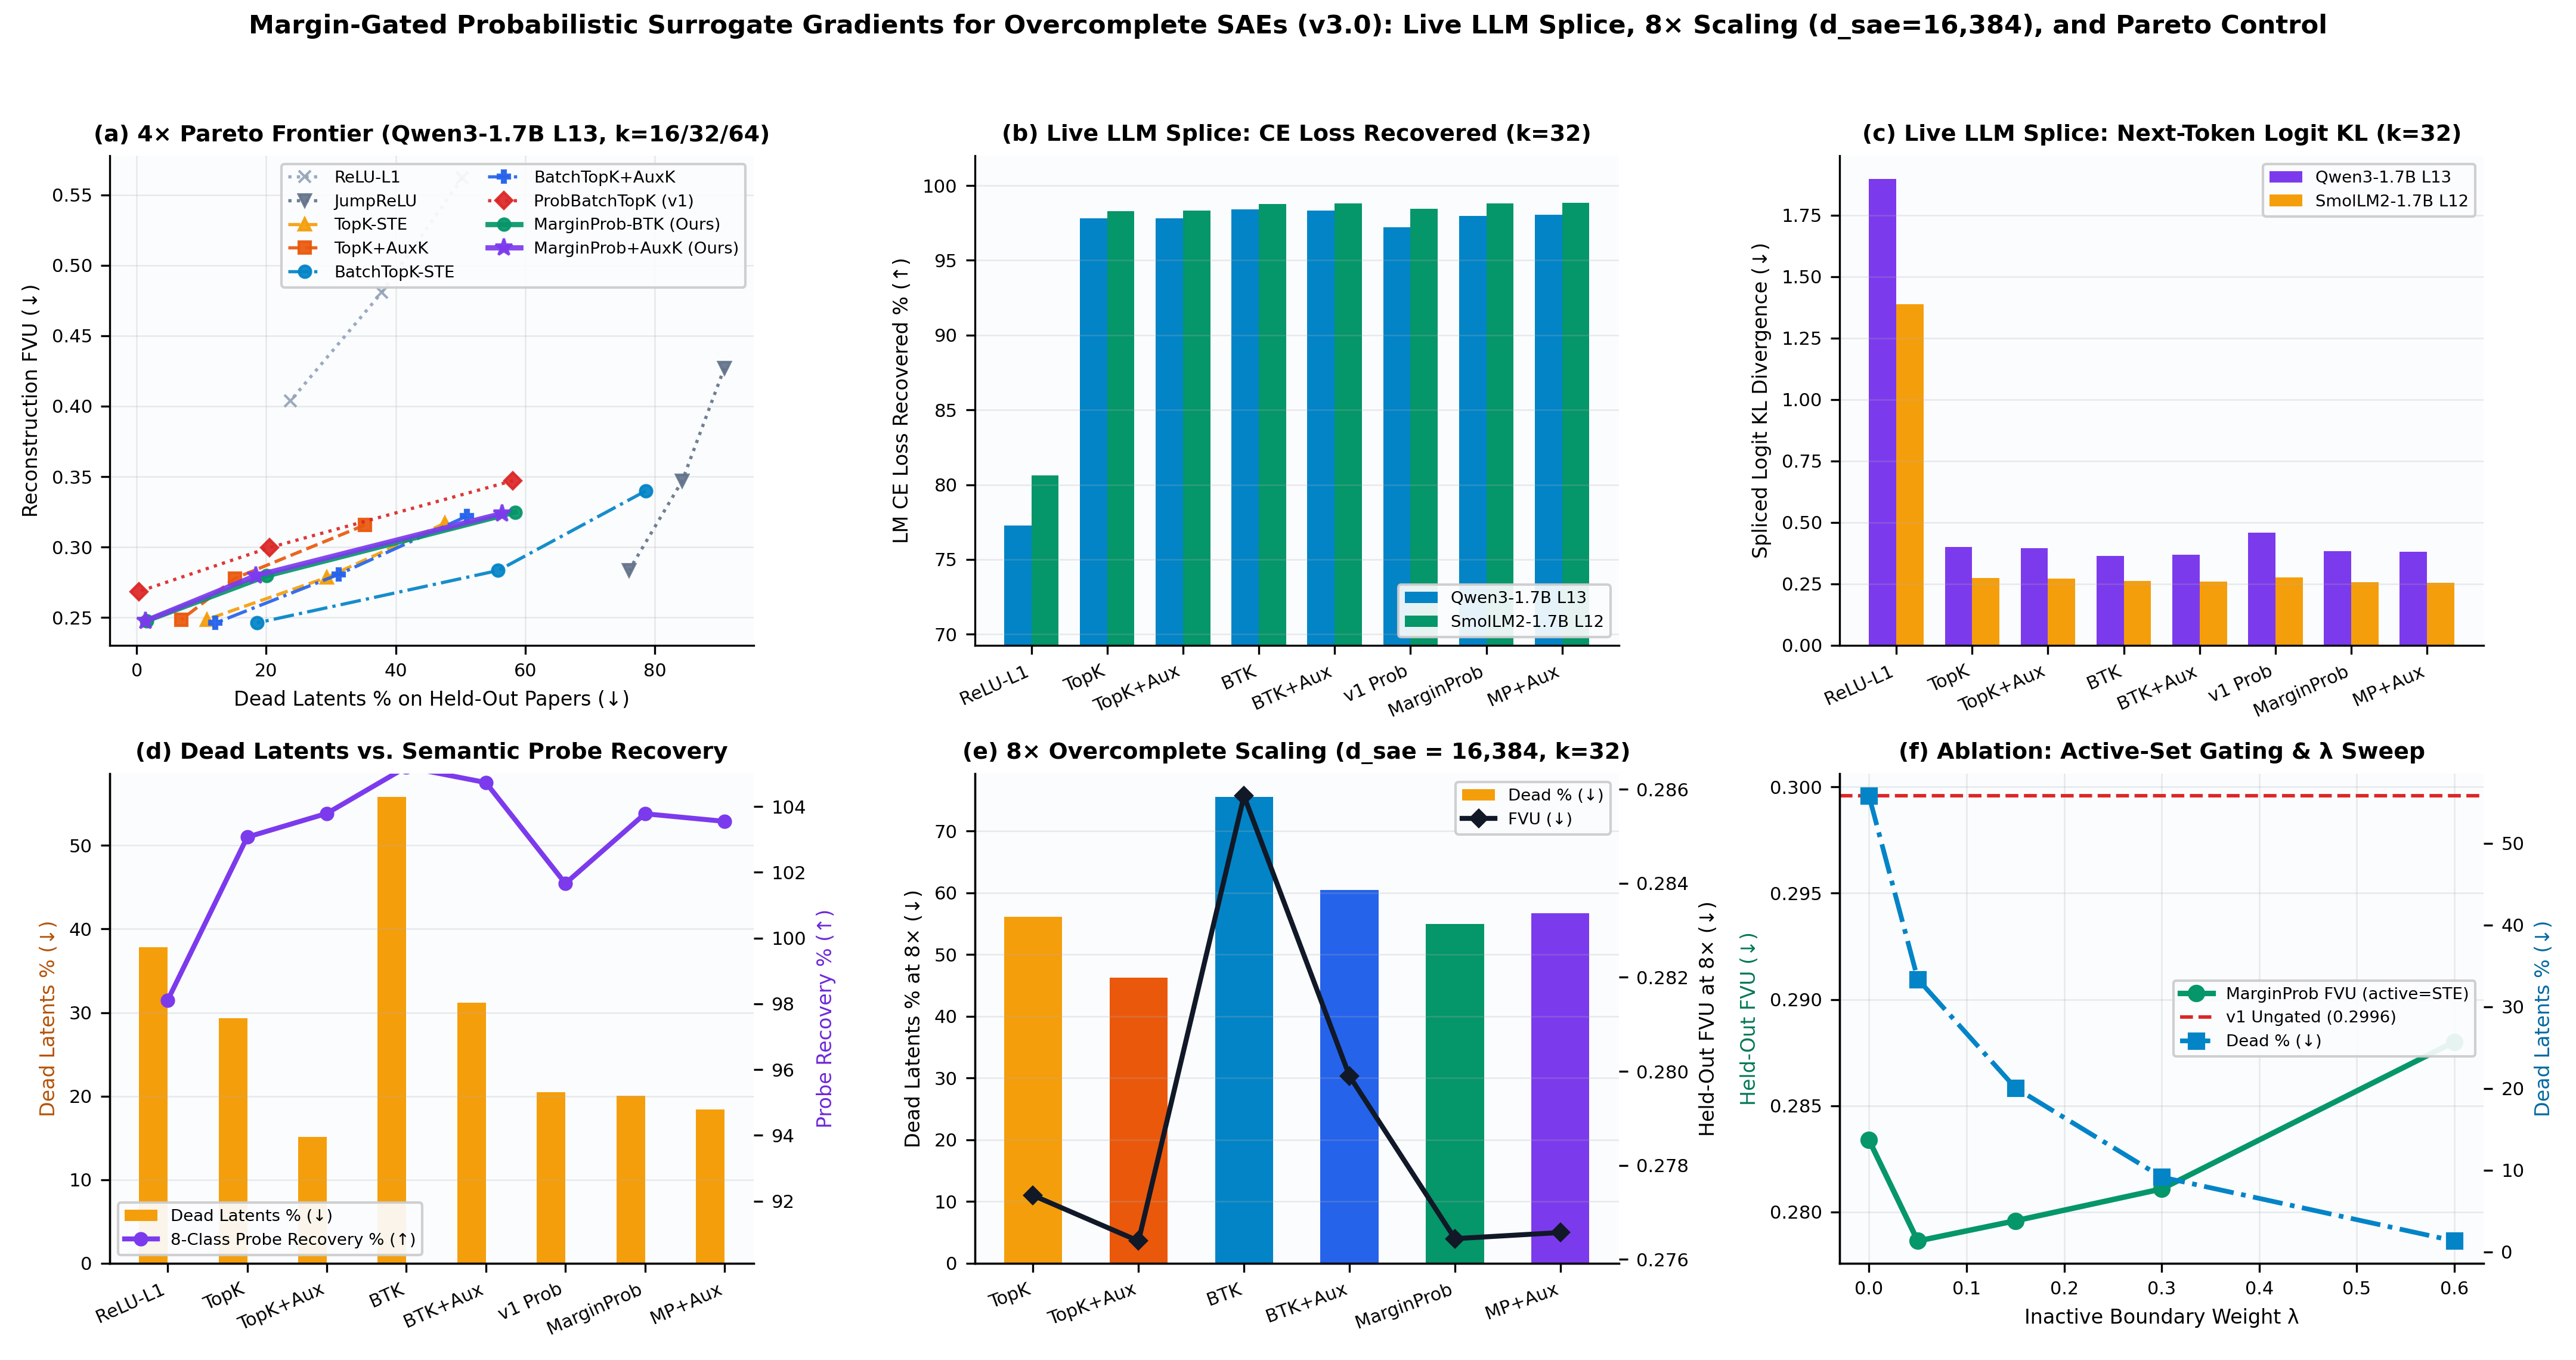
\includegraphics[width=\linewidth]{figure1.png}
  \caption{Version 3.0 SAE benchmark on NVIDIA GeForce RTX 5090: (a) $4\times$ FVU vs.\ dead-latent Pareto frontier ($k \in \{16,32,64\}$); (b--c) Live transformer causal splice CE Loss Recovered \% and Logit KL ($k=32$); (d) Dead latents vs.\ 8-class probe recovery; (e) $8\times$ overcomplete scaling ($d_{\mathrm{sae}}=16{,}384$); (f) Boundary weight $\lambda$ ablation.}
  \label{fig:sae_main}
\end{figure*}

\begin{table*}[t]
  \centering
  \caption{Primary $4\times$ overcomplete SAE benchmark ($d_{\mathrm{sae}}=8{,}192, k=32$, 3 seeds) on paper-disjoint held-out tokens, including live transformer causal splice CE Loss Recovered \%, next-token Logit KL, 8-class probe recovery, and capacity-controlled Top-512 Hungarian cross-seed cosine.}
  \label{tab:sae_main}
  \setlength{\tabcolsep}{3.2pt}
  \scriptsize
  \resizebox{\linewidth}{!}{\begin{tabular}{llrrrrrr}
    \toprule
    Model & Method & FVU ($\downarrow$) & Dead \% ($\downarrow$) & CE Rec \% ($\uparrow$) & Logit KL ($\downarrow$) & Probe Rec ($\uparrow$) & Top-512 Hung \\
    \midrule
        Qwen3-1.7B & ReLU-$L_1$ \citep{bricken2023monosemanticity} & $0.4807\pm0.0016$ & 37.83\% & 77.26\% & 1.8969 & 98.1\% & 0.525 \\
    Qwen3-1.7B & JumpReLU \citep{rajamanoharan2024jumprelu} & $0.3472\pm0.0028$ & 84.22\% & 95.90\% & 0.5866 & 100.7\% & 0.480 \\
    Qwen3-1.7B & TopK-STE \citep{gao2024scaling} & $0.2784\pm0.0003$ & 29.32\% & 97.81\% & 0.3991 & 103.1\% & 0.494 \\
    Qwen3-1.7B & TopK+AuxK \citep{gao2024scaling} & $0.2778\pm0.0001$ & 15.13\% & 97.82\% & 0.3959 & 103.8\% & 0.499 \\
    Qwen3-1.7B & BatchTopK-STE \citep{bussmann2024batchtopk} & $0.2834\pm0.0015$ & 55.80\% & 98.42\% & 0.3623 & 105.2\% & 0.500 \\
    Qwen3-1.7B & BatchTopK+AuxK \citep{bussmann2024batchtopk} & $0.2806\pm0.0011$ & 31.15\% & 98.33\% & 0.3691 & 104.7\% & 0.503 \\
    Qwen3-1.7B & ProbBatchTopK (v1 Ungated) & $0.2996\pm0.0003$ & 20.48\% & 97.20\% & 0.4582 & 101.7\% & 0.483 \\
    Qwen3-1.7B & \textbf{MarginProb-BatchTopK (Ours)} & $0.2796\pm0.0007$ & 20.07\% & 97.96\% & 0.3819 & 103.8\% & 0.502 \\
    Qwen3-1.7B & \textbf{MarginProb+AuxK (Ours)} & $0.2797\pm0.0005$ & 18.39\% & 98.04\% & 0.3796 & 103.5\% & 0.498 \\
    \midrule
    SmolLM2-1.7B & ReLU-$L_1$ \citep{bricken2023monosemanticity} & $0.4935\pm0.0147$ & 19.84\% & 80.61\% & 1.3876 & 102.3\% & 0.402 \\
    SmolLM2-1.7B & JumpReLU \citep{rajamanoharan2024jumprelu} & $0.3663\pm0.0129$ & 88.55\% & 95.59\% & 0.4711 & 103.0\% & 0.480 \\
    SmolLM2-1.7B & TopK-STE \citep{gao2024scaling} & $0.2670\pm0.0002$ & 31.42\% & 98.28\% & 0.2735 & 107.1\% & 0.509 \\
    SmolLM2-1.7B & TopK+AuxK \citep{gao2024scaling} & $0.2659\pm0.0001$ & 18.17\% & 98.32\% & 0.2723 & 105.8\% & 0.509 \\
    SmolLM2-1.7B & BatchTopK-STE \citep{bussmann2024batchtopk} & $0.2761\pm0.0027$ & 49.28\% & 98.75\% & 0.2612 & 107.1\% & 0.485 \\
    SmolLM2-1.7B & BatchTopK+AuxK \citep{bussmann2024batchtopk} & $0.2729\pm0.0024$ & 30.23\% & 98.79\% & 0.2598 & 106.6\% & 0.493 \\
    SmolLM2-1.7B & ProbBatchTopK (v1 Ungated) & $0.2826\pm0.0006$ & 18.10\% & 98.46\% & 0.2753 & 107.1\% & 0.498 \\
    SmolLM2-1.7B & \textbf{MarginProb-BatchTopK (Ours)} & $0.2720\pm0.0023$ & 31.33\% & 98.82\% & 0.2561 & 108.6\% & 0.495 \\
    SmolLM2-1.7B & \textbf{MarginProb+AuxK (Ours)} & $0.2719\pm0.0021$ & 29.02\% & 98.85\% & 0.2552 & 107.6\% & 0.490 \\
    \bottomrule
  \end{tabular}}
\end{table*}

\begin{table*}[t]
  \centering
  \caption{Sparsity-budget scaling across $k \in \{16,32,64\}$ ($d_{\mathrm{sae}}=8{,}192$, 3 seeds) on both LLM families.}
  \label{tab:sae_k}
  \scriptsize
  \resizebox{\linewidth}{!}{\begin{tabular}{llrrrr}
    \toprule
    $k$ & Method & Qwen3 FVU ($\downarrow$) & Qwen3 Dead \% ($\downarrow$) & SmolLM2 FVU ($\downarrow$) & SmolLM2 Dead \% ($\downarrow$) \\
    \midrule
        $k=16$ & TopK-STE \citep{gao2024scaling} & 0.3168 & 47.55\% & 0.3060 & 48.87\% \\
    $k=16$ & TopK+AuxK \citep{gao2024scaling} & 0.3157 & 35.24\% & 0.3038 & 36.54\% \\
    $k=16$ & BatchTopK-STE \citep{bussmann2024batchtopk} & 0.3398 & 78.56\% & 0.3289 & 73.68\% \\
    $k=16$ & BatchTopK+AuxK \citep{bussmann2024batchtopk} & 0.3220 & 50.97\% & 0.3134 & 46.89\% \\
    $k=16$ & ProbBatchTopK (v1 Ungated) & 0.3472 & 58.10\% & 0.3291 & 54.95\% \\
    $k=16$ & \textbf{MarginProb-BatchTopK (Ours)} & 0.3248 & 58.45\% & 0.3208 & 61.99\% \\
    $k=16$ & \textbf{MarginProb+AuxK (Ours)} & 0.3239 & 56.40\% & 0.3185 & 54.40\% \\
    \midrule
    $k=32$ & TopK-STE \citep{gao2024scaling} & 0.2784 & 29.32\% & 0.2670 & 31.42\% \\
    $k=32$ & TopK+AuxK \citep{gao2024scaling} & 0.2778 & 15.13\% & 0.2659 & 18.17\% \\
    $k=32$ & BatchTopK-STE \citep{bussmann2024batchtopk} & 0.2834 & 55.80\% & 0.2761 & 49.28\% \\
    $k=32$ & BatchTopK+AuxK \citep{bussmann2024batchtopk} & 0.2806 & 31.15\% & 0.2729 & 30.23\% \\
    $k=32$ & ProbBatchTopK (v1 Ungated) & 0.2996 & 20.48\% & 0.2826 & 18.10\% \\
    $k=32$ & \textbf{MarginProb-BatchTopK (Ours)} & 0.2796 & 20.07\% & 0.2720 & 31.33\% \\
    $k=32$ & \textbf{MarginProb+AuxK (Ours)} & 0.2797 & 18.39\% & 0.2719 & 29.02\% \\
    \midrule
    $k=64$ & TopK-STE \citep{gao2024scaling} & 0.2486 & 10.84\% & 0.2388 & 12.72\% \\
    $k=64$ & TopK+AuxK \citep{gao2024scaling} & 0.2485 & 6.90\% & 0.2380 & 8.45\% \\
    $k=64$ & BatchTopK-STE \citep{bussmann2024batchtopk} & 0.2462 & 18.58\% & 0.2390 & 22.06\% \\
    $k=64$ & BatchTopK+AuxK \citep{bussmann2024batchtopk} & 0.2461 & 12.17\% & 0.2392 & 15.61\% \\
    $k=64$ & ProbBatchTopK (v1 Ungated) & 0.2685 & 0.37\% & 0.2523 & 0.30\% \\
    $k=64$ & \textbf{MarginProb-BatchTopK (Ours)} & 0.2477 & 1.53\% & 0.2402 & 5.16\% \\
    $k=64$ & \textbf{MarginProb+AuxK (Ours)} & 0.2476 & 1.38\% & 0.2402 & 5.26\% \\
    \bottomrule
  \end{tabular}}
\end{table*}

\begin{table*}[t]
  \centering
  \caption{$8\times$ overcomplete scaling ($d_{\mathrm{in}}=2{,}048 \to d_{\mathrm{sae}}=16{,}384, k=32$, 3 seeds) on Qwen3-1.7B L13.}
  \label{tab:sae_8x}
  \scriptsize
  \begin{tabular}{lrrr}
    \toprule
    Method ($8\times$ Width, $d_{\mathrm{sae}}=16{,}384$) & FVU ($\downarrow$) & Dead Latents \% ($\downarrow$) & Util.\ Entropy ($\uparrow$) \\
    \midrule
        TopK-STE \citep{gao2024scaling} & $0.2774\pm0.0006$ & $56.06\%\pm0.29\%$ & 0.8169 \\
    TopK+AuxK \citep{gao2024scaling} & $0.2764\pm0.0001$ & $46.27\%\pm0.07\%$ & 0.8163 \\
    BatchTopK-STE \citep{bussmann2024batchtopk} & $0.2859\pm0.0013$ & $75.50\%\pm6.91\%$ & 0.7707 \\
    BatchTopK+AuxK \citep{bussmann2024batchtopk} & $0.2799\pm0.0010$ & $60.44\%\pm1.07\%$ & 0.7794 \\
    \textbf{MarginProb-BatchTopK (Ours)} & $0.2764\pm0.0002$ & $54.89\%\pm0.60\%$ & 0.8020 \\
    \textbf{MarginProb+AuxK (Ours)} & $0.2766\pm0.0002$ & $56.67\%\pm0.89\%$ & 0.8036 \\
    \bottomrule
  \end{tabular}
\end{table*}

\begin{table*}[t]
  \centering
  \caption{Hyperparameter ablation on Qwen3-1.7B L13 ($k=32, d_{\mathrm{sae}}=8{,}192$, 3 seeds). Setting $\lambda=0$ recovers exact BatchTopK-STE.}
  \label{tab:sae_ablation}
  \scriptsize
  \begin{tabular}{llrrr}
    \toprule
    Axis & Setting & FVU ($\downarrow$) & Dead \% ($\downarrow$) & Util.\ Entropy ($\uparrow$) \\
    \midrule
        Boundary weight $\lambda$ & $\lambda=0.00$ & $0.2834\pm0.0015$ & 55.80\% & 0.8365 \\
    Boundary weight $\lambda$ & $\lambda=0.05$ & $0.2786\pm0.0007$ & 33.37\% & 0.8563 \\
    Boundary weight $\lambda$ & $\lambda=0.15$ & $0.2796\pm0.0007$ & 20.07\% & 0.8692 \\
    Boundary weight $\lambda$ & $\lambda=0.30$ & $0.2811\pm0.0007$ & 9.14\% & 0.8875 \\
    Boundary weight $\lambda$ & $\lambda=0.60$ & $0.2880\pm0.0004$ & 1.32\% & 0.9181 \\
    \midrule
    Rel.\ temp.\ $\tau_{\mathrm{rel}}$ & $\tau_{\mathrm{rel}}=0.15$ & 0.2818 & 33.97\% & 0.8689 \\
    Rel.\ temp.\ $\tau_{\mathrm{rel}}$ & $\tau_{\mathrm{rel}}=0.35$ & 0.2796 & 20.07\% & 0.8692 \\
    Rel.\ temp.\ $\tau_{\mathrm{rel}}$ & $\tau_{\mathrm{rel}}=0.70$ & 0.2784 & 23.87\% & 0.8629 \\
    \bottomrule
  \end{tabular}
\end{table*}

\paragraph{Active-Set Gating, Live Causal Splice, and $8\times$ Scaling (Tables~\ref{tab:sae_main}--\ref{tab:sae_8x}).} Across all 18 paired $4\times$ runs, active-set gating removes ungated v1's FVU penalty ($\Delta\mathrm{FVU} = -0.01569$, $p=1.95e-09$) and strictly Pareto-dominates pure-MSE BatchTopK-STE ($\Delta\mathrm{FVU} = -0.00470$, $p=4.10e-03$; dead latents $-19.90$\,pp, $p=7.69e-09$). Spliced live into SmolLM2-1.7B L12, MarginProb+AuxK (98.85\% CE, KL 0.2552) and pure-MSE MarginProb (98.82\%, KL 0.2561) rank \#1 and \#2 across all 9 methods; on Qwen3-1.7B L13, MarginProb recovers 97.96\% CE (KL 0.3819), fully repairing ungated v1 (97.20\%) while cutting dead latents 2.8$\times$ vs.\ BatchTopK-STE (98.42\%, 55.8\% dead). At $8\times$ width ($d_{\mathrm{sae}}=16{,}384$), pure-MSE MarginProb ties TopK+AuxK for the lowest FVU (0.2764) while cutting dead latents from 75.5\% (BatchTopK-STE) and 60.4\% (BatchTopK+AuxK) down to 54.9\%.

\paragraph{Capacity-Controlled Cross-Seed Stability \& Ablations (Tables~\ref{tab:sae_main}, \ref{tab:sae_ablation}).} Evaluating 1-to-1 Hungarian matching on the top-512 most active latents resolves the alive-set capacity confound of raw Hungarian matching: MarginProb matches or exceeds BatchTopK+AuxK and TopK+AuxK across both models (reaching 0.426 vs.\ 0.410 BatchTopK+AuxK at $k=64$). Sweeping $\lambda \in [0, 0.60]$ cuts dead latents monotonically from 55.8\% to 1.32\% (42$\times$ reduction) with an FVU optimum at $\lambda=0.05$ (0.2786).

\section{Limitations and Broader Impact}
(1) Because the hard forward pass zeroes inactive activations, MarginProb routes gradients into $W_{\mathrm{enc}}, b_{\mathrm{enc}}$ without updating $W_{\mathrm{dec}}$ on deeply dead features; combining with AuxK recovers both regimes. (2) While we scale to $8\times$ ($d_{\mathrm{sae}}=16{,}384$) over 205,883 tokens, production 65k--131k SAEs over $10^8+$ tokens warrant future verification. (3) Downstream semantics are evaluated via live LM causal splice and 8-class probes rather than LLM-as-a-judge auto-interpretability. Improving sparse feature dictionaries supports safer, more transparent LLM auditing.

\bibliographystyle{tmlr}
\bibliography{references}
\end{document}
